
\PassOptionsToPackage{full}{textcomp}
\documentclass[]{tufte-handout}
%\usepackage{fontspec}
%\usepackage{ETbb}


% load babel package and options here
%\usepackage[p,osf]{ETbb} % osf in text, tabular lining figures in math
\usepackage{ETbb} % osf in text, tabular lining figures in math
\usepackage[scaled=.95,type1]{cabin} % sans serif in style of Gill Sans
\usepackage[varqu,varl]{zi4}% inconsolata typewriter
\usepackage[T1]{fontenc} % LY1 also works
\usepackage[libertine,vvarbb]{newtxmath}
%\usepackage[cal=boondoxo,bb=boondox,frak=boondox]{mathalfa}

%\geometry{showframe} % display margins for debugging page layout

\usepackage{graphicx} % allow embedded images
%  \setkeys{Gin}{width=\linewidth,totalheight=\textheight,keepaspectratio}
  \graphicspath{{graphics/}} % set of paths to search for images
\usepackage{amsmath}  % extended mathematics
\usepackage{booktabs} % book-quality tables
%\usepackage{units}    % non-stacked fractions and better unit spacing
\usepackage{multicol} % multiple column layout facilities
\usepackage{multirow} % multiple column layout facilities
\usepackage{lipsum}   % filler text
\usepackage{fancyvrb} % extended verbatim environments
  \fvset{fontsize=\normalsize}% default font size for fancy-verbatim environments
\usepackage{gensymb} % provides symbols like \degree
\usepackage{ragged2e} % enables hyphenation in ragged-right justification
\usepackage[normalize-symbols]{textalpha} %enables \textalpha for alpha symbol etc.

\usepackage{hyperref} % enables styling of href and url
\hypersetup{
    pdftitle={Tutorial 3},
    pdfauthor={Barry Linkletter},
    colorlinks=true,
    linkcolor=blue,
    filecolor=magenta,      
    urlcolor=blue,
    pdfborder={0 0 0},
    frenchlinks=false,
    pdfpagemode=FullScreen,
    }

\usepackage{enumitem} % allows resuming enumerate lists.
\usepackage{mathtools}
\usepackage{mhchem}

\usepackage{siunitx} % provides "S" column class for aligning decimals.  


\usepackage{nicefrac}

\usepackage{varioref}

\usepackage{babel}
\usepackage{float}
\usepackage{stackrel}


\usepackage[shortconst]{physconst}

\usepackage[normalem]{ulem}  % provides strikethrough \sout{}

\usepackage{newfloat}
\DeclareFloatingEnvironment[
  fileext = los ,
  listname = {List of Schemes} ,
  name = Scheme
]{scheme}                    % provides scheme numbering for chemical schemes



\newcommand{\Km}{$\rm K_M$}
\newcommand{\Vmax}{$\rm V_{max}$}
\newcommand{\kcat}{$\rm k_{cat}$}



\title{Exploration \#X: Searching for a Synthesis Enzyme}
\author[Barry Linkletter]{Barry Linkletter}
\date{} % without \date command, current date is supplied


\begin{document}
\justifying


\maketitle% this prints the handout title, author, and date

\begin{abstract}
\noindent Enzymes can be recruited to perform reactions in the service of organic chem\-istry. Can we find a mutant of  \emph{\textbeta -galactosidase} that will enable us to produce a gly\-cos\-yl\-at\-ed polyphenolic nutraceutical?
\marginnote[-20mm]{This document was produced using the \LaTeX\ typesetting language with the Tufte-handout document class. Images of proteins were created using \textit{UCSF Chimera}. Chemical diagrams were made with \textit{ChemDoodle} and further edited with \textit{Affinity Designer}.}

\end{abstract}





\section{Enzymes Kinetics and Synthesis}

\begin{marginfigure}[5mm]

  \caption[0mm]{The natural products daidzin and daidzein compared to our synthetic target, 7-(\textbeta -D-Galactopyranosyloxy)-4'-hydroxyisoflavone} 
  \vspace{4mm}
    \centering
  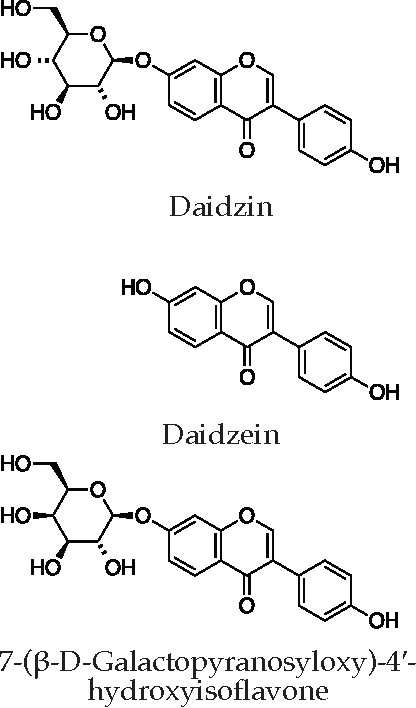
\includegraphics[scale=0.6]{Daidzin2.pdf}
  \vspace{5mm}
  \label{fig:fig1}
\end{marginfigure}




Enzymes catalyze many biological reactions. Often the reaction catalyzed is a desirable synthetic reaction. The stereospecificity and high catalytic efficiency of enzymes makes them prime candidates for use in organic synth\-es\-is. In this exercise we will choose a target reaction, find an enzyme that can catalyze the reaction and then attempt to improve the enzyme by generating mutants. We will observe the reaction kinetics of the enzyme candidates using an assay reaction and explore the use of computational tools to deal with large amounts of data.

\section{A Desirable Reaction}

Daidzin is a natural product found in Japanese kudzo vines and soybeen leaves. It is believed to be the active ingredient in herbal medicinal extracts that have been used to treat alcoholism over hundreds of years. Toxic alcohol is removed from the body by the action of \emph{alcohol dehydrogenase}, which cata\-lyz\-es the oxidation of alcohol by NAD\textsuperscript{+} to give acetaldehyde, an even more toxic substance. Another enzyme, \emph{aldehyde de\-hy\-drog\-en\-ase}, quick\-ly oxid\-izes the aldehyde to give acetic acid that can be ligated to coenzyme-A and used for energy or, more likely, to make fats. Daidzin inhibits \emph{aldehyde de\-hy\-drog\-en\-ase} and this will allow acetaldehyde to build up and make a person very uncomfortable.\sidenote[][-8mm]{
``Daidzin: A Potent, Selective Inhibitor of Human Mitochondrial Aldehyde Dehydrogenase.'' W.-M. Keung, B.L. Vallee, \emph{Proc. Natl. Acad. Sci. USA}, \textbf{1993}, \emph{90}, 1247–1251. \url{https://www.jstor.org/stable/2361166}\vspace{2mm}}\textsuperscript{,}\sidenote[][0mm]{``Structure of Daidzin, a Naturally Occurring Anti-Alcohol-Addiction Agent in Complex with Human Mitochondrial Aldehyde Dehydrogenase.'' E.D. Lowe et al., \emph{J. Med. Chem.}, \textbf{2008}, \emph{51}, 4482-4487. \url{https://doi.org/10.1021/jm800488j}\vspace{2mm}}
 

Natural products can be expensive to extract and often the extraction method degrades the material. I have found a cheap source of a related compound, daidzein, from coal tar. This simpler compound is also an inhib\-itor of \emph{aldehyde de\-hy\-drog\-en\-ase} but it is not soluble in water without the sugar group. I want to glycosylate the daidzein with galactose, rather than the glucose that is present in daidzin. I plan to use an enzyme to catalyze the condensation reaction.

\begin{figure}[h!]

  \caption[0mm]{Condensation of a hemiacetal with a phenol in the synthesis of  7-(\textbeta -D-Galactopyranosyloxy)-4'-hydroxyisoflavone} 
  \vspace{2mm}
    \centering
  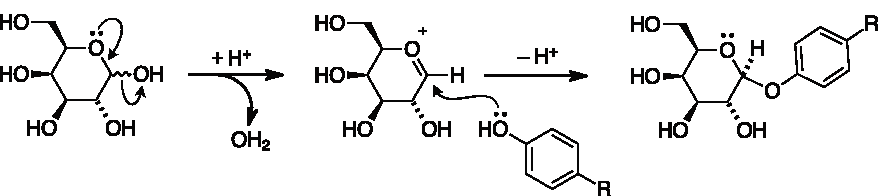
\includegraphics[scale=0.6]{reaction1.pdf}
  \vspace{5mm}
  \label{fig:fig2}
\end{figure}

Using galactose will give us a novel compound that can be patented. Daid\-zein and galactose are found in foodstuffs and enzymes are a natural material so I plan to simplify the regulatory regime by classifying my molecule as a ``nutraceutical'', a food-based drug with which humanity is already exper\-i\-enced.\sidenote[][0mm]{``The current use and evolving landscape of nutraceuticals.'' Avijeet S. Chopra et al., \textit{Pharmacological Research}, \textbf{2022}, \textit{175}, 106001, \url{https://doi.org/10.1016/j.phrs.2021.106001}} This will greatly reduce my costs in achieving regulatory approval. My lawyer is working on it.

\section{The Chosen Enzyme}

I plan to use \emph{\textbeta -galactosidase} as a catalyst for my condensation reaction.\sidenote[][0mm]{``\emph{lacZ} \emph{\textbeta -galactosidase}: Structure and function of an enzyme of historical and molecular biological importance.'' D.H. Juers, B.W. Matthews, R.E. Huber, \emph{Protein Sci.}, \textbf{2012}, \emph{21}, 1792-1807. \url{https://doi.org/10.1002/pro.2165}\vspace{2mm}} It is an enzyme that catalyzes the hydrolysis of the glycosidic bond between \textbeta -galactose and glucose (in lactose). It can also catalyze the reverse and is observed to produce allolactose in natural systems from galactose and glucose. Allolactose is a potent inducer for the \emph{lacZ} gene that produces \emph{\textbeta -galactosidase}.


\begin{figure}[h!]

  \caption[0mm]{Hydrolysis of lactose by \emph{\textbeta -galactosidase}. The enzyme catalyzes the formation of and stabilizes the cationic intermediate. The water can add, completing the hydrolysis reaction, or another nucleophile can add to make a different glycoside.} 
  \vspace{2mm}
    \centering
  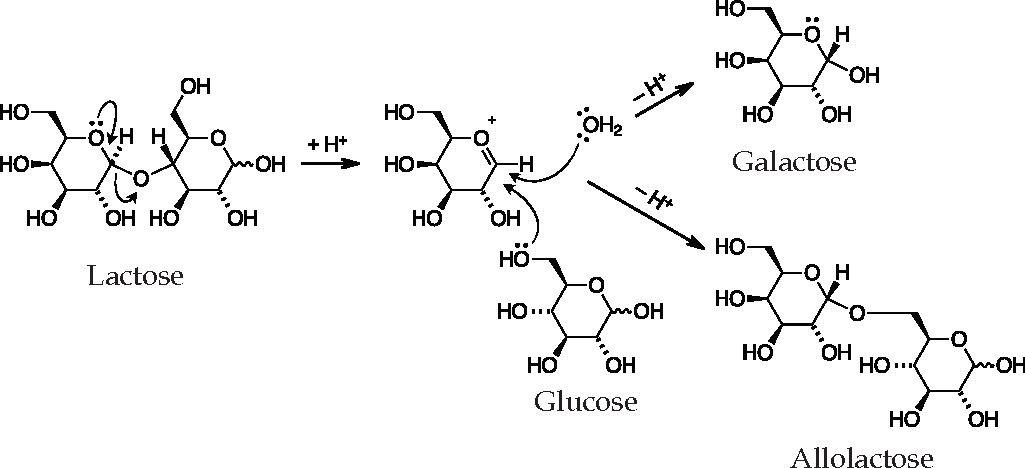
\includegraphics[scale=0.6]{enzreaction1.pdf}
  \vspace{5mm}
  \label{fig:fig3}
\end{figure}

\emph{\textbeta -galactosidase} has been used for this type of synthetic chemistry over the past few decades with middling success. Recent work on making phenyl ethers has encouraged me to try this approach.\sidenote[][-20mm]{``Conventional and non-conventional applications of \emph{\textbeta -galactosidases}.'' C. Vera et al., \emph{Biochim. Biophys. Acta Proteins Proteom.}, \textbf{2020}, \emph{1868}, 140271. \url{https://doi.org/10.1016/j.bbapap.2019.140271}\vspace{2mm}}\textsuperscript{,}\sidenote[][0mm]{``Glycosylation of phenolic compounds by the site-mutated \emph{\textbeta -galactosidase} from \emph{lactobacillus bulgaricus L3}.'' L. Lu et al., \emph{PLoS ONE}, \textbf{2015}, \emph{10}, e0121445. \url{https://doi.org/10.1371/journal.pone.0121445}\vspace{2mm}}

\section{Finding the One}

Initially we must find a version of \emph{\textbeta -galactosidase} that will hold a phenol \textbeta -galactoside in its active site. An enzyme that can effectively catalyze the hydrolysis of the target may be the best at catalyzing the reverse reaction when we optimize conditions to favour condensation (I know, we must find a way to exclude water from the system - a tall order for enzyme chemistry. I plan to use modern methods involving ionic liquids rather than water as the solvent.\sidenote[][-10mm]{``Facilitating enzymatic reactions by using ionic liquids: A mini review.'' A.M. Amal et al., \emph{Curr. Opin. Green Sustain. Chem.}, \textbf{2021}, \emph{}27, 100406, \url{https://doi.org/10.1016/j.cogsc.2020.100406}\vspace{2mm}} It's called research for a reason.)

\section{The Experiment}

I will obtain cells that express various versions of \emph{\textbeta -galactosidase} that have been modified with an affinity tag for easy and selective purification. I will expose these cells to various mutagens and then isolate single colonies that retain \emph{\textbeta -galactosidase} activity. I will grow up each cell line and then extract proteins from the cells.  I will isolate the \emph{\textbeta -galactosidase} by using an affinity column and then separate the enzyme from the release buffer with a size-exclusion spin column. The concentration of protein will be determined by spectrophotometry. I will dilute the samples to obtain an enzyme con\-cen\-tra\-tion of \qty{10}{nM}. Each sample will be flash frozen in liquid nitrogen and stored in a \qty{-80}{\degreeCelsius} freezer.

The assay reaction will follow the release of p-nitrophenolate anion from p-Nitrophenyl-\textbeta -\textsc{d}-galactoside (PNP-\textbeta-D-Gal).\sidenote[][-15mm]{``Recent advances in enzyme assays.'' J.-P. Goddard, J.-L. Reymond, \emph{Trends Biotech.}, \textbf{2004}, \emph{22}, 363-370. \url{https://doi.org/10.1016/j.tibtech.2004.04.005}\vspace{2mm} }\textsuperscript{,}\sidenote[][0mm]{``Enzyme assays for high-throughput screening.'' J.-P. Goddard, J.-L. Reymond, \emph{Curr. Opin. Biotech.}, \textbf{2004}, \emph{15}, 314-322. \url{https://doi.org/10.1016/j.copbio.2004.06.008.}\vspace{2mm}}\textsuperscript{,}\sidenote[][0mm]{``Enzyme assays.'' H. Bisswanger, \emph{Perspectives in Science}, \textbf{2014}, \emph{1}, 41-55. \url{https://doi.org/10.1016/j.pisc.2014.02.005}\vspace{2mm}} I will use a microtitre plate and a plate reader to conduct my assays. Each column in a plate will contain a given sample of enzyme and each row will have a set concentration of substrate.

The workflow will feature a robotic liquid-handling system\sidenote[][0mm]{Consider the \href{https://www.hamiltoncompany.com/automated-liquid-handling/platforms/microlab-prep}{MicroLab-Prep robot from Hamilton Co.} as an example.} to set up a 96-well plate with the various enzyme samples and a separate 96-well plate with the various substrate samples. I will use  96-well multichannel pipette system\sidenote[][0mm]{Consider the \href{https://www.integra-biosciences.com/canada/en/electronic-pipettes/viaflo-96-viaflo-384}{ViaFlow 96 from Integra Bioscience} for an example.} to transfer the substrate samples to the enzyme samples simultaneously. I then insert the plate in the plate reader\sidenote[][0mm]{Consider the \href{https://www.moleculardevices.com/products/microplate-readers/absorbance-readers/spectramax-abs-plate-readers}{SpectraMax Abs plate reader from Molecular Devices Inc.} as an example.} and begin reading the absorbance at \qty{405}{nm} over time. It took time to start the assay and set the plate in the plate reader so all my measurements will start at the 30-second mark. 

\section{Assay Method}

Each well of the plate contains enough liquid to make a path length of \qty{1}{cm} in the well. After the substrate and enzyme solutions are combined, each well will contain the enzyme and substrate in a \qty{0.100}{M} phosphate buffer set to pH 7.0. Substrate concentration in each row and enzymes in each lane will be recorded in each data file. A sample plate plan is shown below.

\begin{figure}[h!]

  \caption[0mm]{A typical setup for a multiwell plate. Each row contains the same amount of substrate across the width of the plate. Each column has the same amount of a given enzyme in each well. All wells have the same volume, buffer concentration, pH and any other variables constant.} 
  \vspace{2mm}
    \centering
  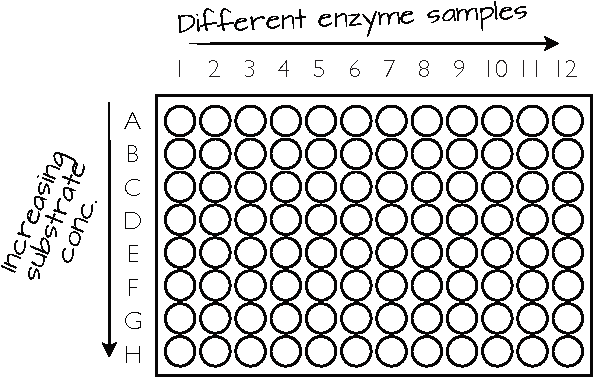
\includegraphics[scale=0.7]{Microtitreplatediagram.pdf}
  \vspace{2mm}
  \label{fig:fig4}
\end{figure}


Each plate was observed for 60 minutes with absorbance recorded every 10 seconds. The data from each plate will be converted to individual csv files containing absorbance vs. time data series for each well in the plate. File names will correspond to the column and rows and inspecting the data folder for each plate will reveal the scheme.

\section{It's Your Job Now}

You are employed at my nimble and agile\sidenote[][0mm]{``Nimble and agile'' is a phrase that means ``could be bankrupt tomorrow'' in business doublespeak.} startup company and you are analyzing data from these assays on our library of purified \emph{\textbeta -galactosidase} sam\-ples. Consider the report that accompanies this document in which your predecessor conducted some initial experiments to determine the best con\-cen\-tra\-tion of enzyme to use in our assays. Your predecessor also conducted all the assays and has collected the data in a series of folders that are included with this exercise. Using the report as a guide and stealing the associated code, analyze the data in the 16 plates that have been recorded and report to me the ten enzyme mutants that have the best $k_{cat}/K_M$ value for our assay reaction. 

You will need to examine the data and adjust the code that you are stealing to work with the data. The initial experiment to determine the optimal enzyme concentration used a slightly different setup in the filenames and arrangement of columns. Once you get the code working for one set of data it should work for all.

Find and identify the top ten. Carefully document the workflow and the changes to the code (you don't need to print out the whole program, just describe what changes you made). We have purchased the robotic pipettors described above and will soon be giving you dozens of plates to analyze each day. You code could become an automated analysis system as well with some improvements but for now it does not matter if you need to manually run the code on each set of data.

\section{Your Report} 

Your report should describe the improvements and changes that you had to make to the code and explain how to use the code (e.g. ``change the file name to the next filename and then run the whole thing again.''). Then you should present how the plates were set up (the 16 plates that you will be analyzing are all set up the same so one explanation will do for all) and present a table that reports the $k_{cat}/K_M$ values with the standard deviation for every enzyme (there will be 176 different Michaelis-Menten plots in your analysis so you will be reporting the $k_{cat}/K_M$ values from 176 experiments with mutant enzymes. Then pick out the ten best values and make a new table of that data. If any of those ten show promise in the initial trials for glycosylation of isoflavone in ionic liquid solvents than we will send them off for sequencing and perhaps use the bacterial cell lines as starting points in our next series of mutations. 

You should include some representative plots that were used to calculate the Michaelis-Menten parameters, \Vmax\ and \Km. Please do not include 176 plots.

This anticipated cycle of mutate, pick the best, mutate again, pick the best, etc. is a form of directed evolution. Is there a more efficient way to do this than exposing bacteria to mutagens? Learn about directed evolution\sidenote[][-10mm]{There are many places to go where you can learn about directed evolution. I usually start at the library. David Goodsell has presented a short essay on the subject: ``Directed Evolution of Enzymes.'' David Goodsell, \emph{Molecule of the Month}, \textbf{2018}, \url{http://doi.org/10.2210/rcsb_pdb/mom_2018_12}} and tell me how I can do all of this faster with fewer employees.


\section{Summary}

I have explained the rational for our plan to assay hundreds of potential mutants of \emph{\textbeta -galactosidase} to find the one that catalyzes the hydrolysis of a phenol glycoside with the greatest efficiency. I hope to use the winning enzyme in the reverse reaction as a tool in organic synthesis. You are to analyze the assay data for \emph{\textbeta -galactosidase} from 176 different cell lines and report the ten best candidates. You are also to write a report so that others can follow your work.\sidenote[][0mm]{No job lasts forever. Learn, gather experience and connections, and always seek to move on and up.} Also, please tell us how we can more efficiently perform our directed evolution experiments so that we can save time and money.



\nobibliography{}

\end{document}